\chapter{Muscles and Joints}\label{ch:g10:muscles-and-joints}

A footballer plants his foot, turns, and goes down clutching his knee.
The diagnosis, an hour later: a torn \omterm{def:g10:muscles-and-joints:joint}{ligament}. Nothing in the bones is
broken, no muscle has failed; a strap of tissue a few centimetres long,
whose job was to hold two bones in line, has given way under a twist it
was never built for. To understand what tore, and why the knee will need
months to recover, we need to know what a \omterm{def:g10:muscles-and-joints:joint}{joint} is made of, how muscles
pull on it, and what forces run through it when a body of seventy
kilograms lands on one leg.

\section{The joint}

\begin{definition}[Joint]\label{def:g10:muscles-and-joints:joint}
A \emph{joint}\index{joint} is the place where two bones meet. In a
mobile joint such as the knee, hip, shoulder or elbow, the ends of the
bones are covered with a layer of smooth \emph{cartilage}\index{cartilage},
a few millimetres thick, and enclosed in a sealed sac, the
\emph{capsule}, whose lining secretes the \emph{synovial fluid} that
lubricates the surfaces. Bands of tough tissue, the
\emph{ligaments}\index{ligament}, run from bone to bone across the
joint and limit its movements to the intended ones. In the knee two
crescents of cartilage, the \emph{menisci}, sit between the bones and
spread the load.
\end{definition}

\begin{omfigure}
\begin{tikzpicture}
  \node[anchor=south west, inner sep=0] (img) at (0,0)
    {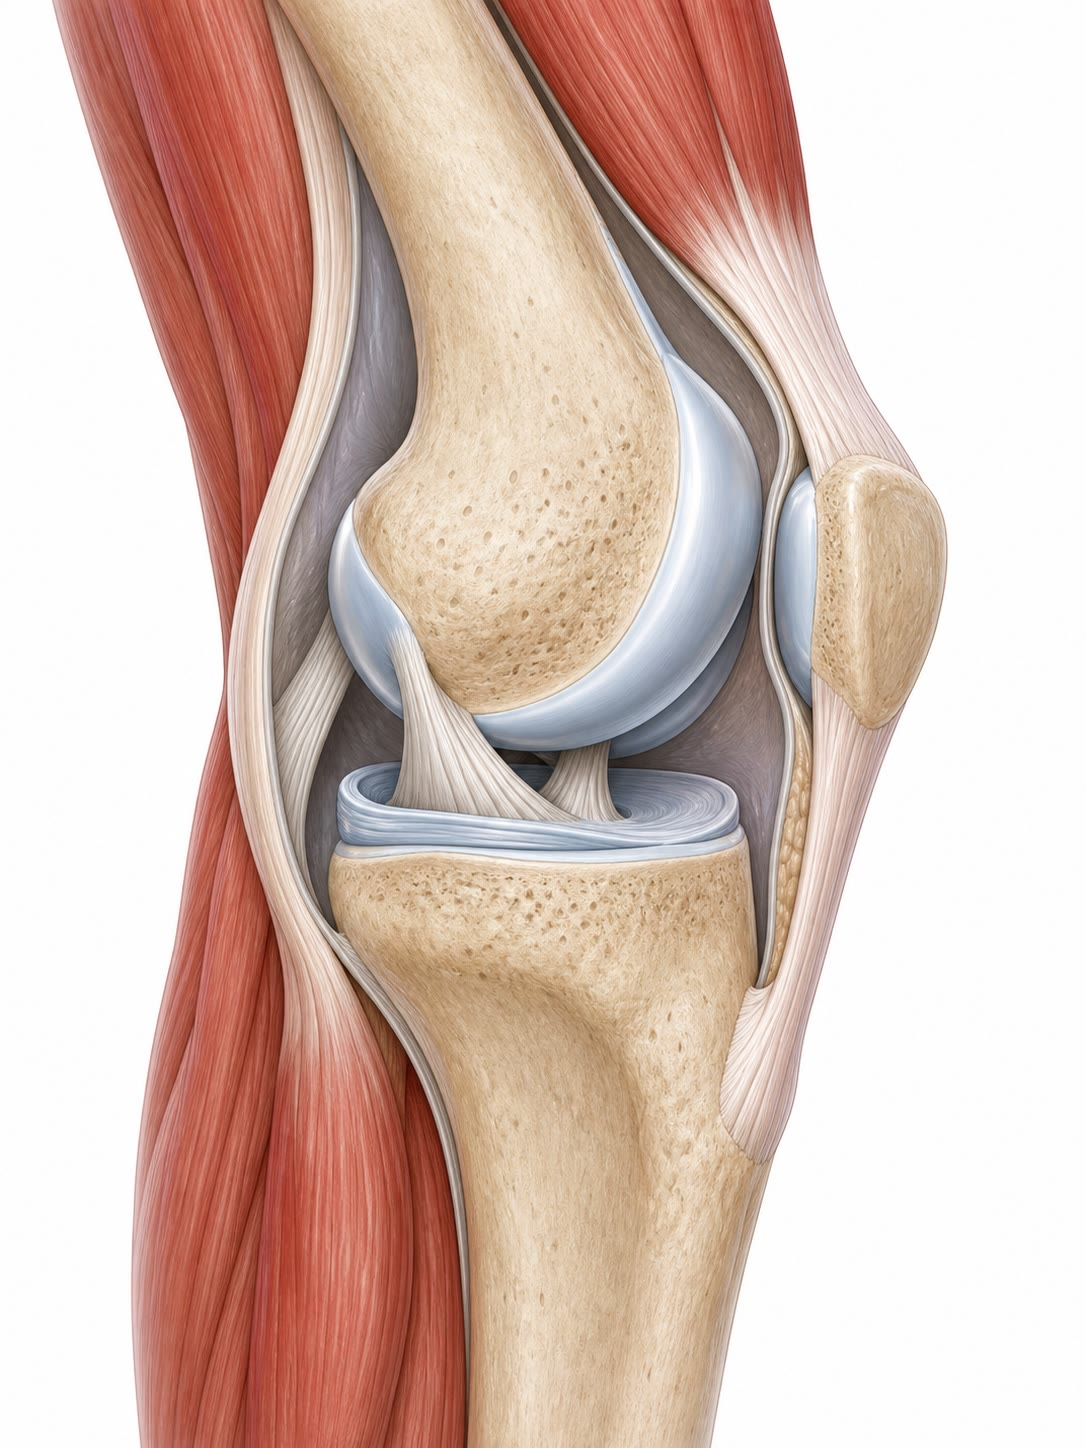
\includegraphics[width=0.4\linewidth]{images/book2/ai/fig-knee-cutaway.jpg}};
  \begin{scope}[x={(img.south east)}, y={(img.north west)},
      every node/.style={font=\small}]
    \draw[omDef, thick] (0.50,0.86) -- (1.05,0.90) node[right] {femur};
    \draw[omDef, thick] (0.76,0.74) -- (1.05,0.74) node[right] {quadriceps tendon};
    \draw[omDef, thick] (0.82,0.58) -- (1.05,0.58) node[right] {patella};
    \draw[omDef, thick] (0.50,0.20) -- (1.05,0.14) node[right] {tibia};
    \draw[omDef, thick] (0.34,0.60) -- (-0.05,0.64) node[left] {cartilage};
    \draw[omDef, thick] (0.50,0.50) -- (-0.05,0.50) node[left] {ligament};
    \draw[omDef, thick] (0.40,0.44) -- (-0.05,0.36) node[left] {meniscus};
  \end{scope}
\end{tikzpicture}

{\small The knee in section: femur above, tibia below, the patella
(kneecap) in front in the \omterm{def:g10:muscles-and-joints:muscle}{tendon} of the thigh muscle; \omterm{def:g10:muscles-and-joints:joint}{cartilage} on the
bone ends, the meniscus between them, \omterm{def:g10:muscles-and-joints:joint}{ligaments} holding the bones
together.}
\end{omfigure}

\begin{proposition}[What each part is for]\label{prop:g10:muscles-and-joints:parts}
\omterm{def:g10:muscles-and-joints:joint}{Cartilage} and synovial fluid make the surfaces slide with less
friction than ice on ice; the menisci distribute a load that would
otherwise concentrate on a few square millimetres; the \omterm{def:g10:muscles-and-joints:joint}{ligaments} allow
the knee to bend and straighten but resist twisting and sideways
bending; the capsule keeps the fluid in. Each part has its own
failure: \omterm{def:g10:muscles-and-joints:joint}{cartilage} wears (arthrosis), a meniscus tears under a twist
with the knee bent, a \omterm{def:g10:muscles-and-joints:joint}{ligament} sprains or ruptures when the \omterm{def:g10:muscles-and-joints:joint}{joint} is
forced beyond its range.
\end{proposition}
\admitted

\begin{example}[Sprain, tear, dislocation]\label{ex:g10:muscles-and-joints:injuries}
Twist an ankle on a kerb: the \omterm{def:g10:muscles-and-joints:joint}{ligaments} on the outside are stretched
beyond their limit --- a \emph{sprain}; the \omterm{def:g10:muscles-and-joints:joint}{joint} swells as the capsule
bleeds and fluid accumulates. Pull hard on a cold hamstring: some of
its fibres rupture --- a muscle \emph{tear}. Fall on an outstretched
arm: the head of the humerus may leave its socket --- a
\emph{dislocation}, the \omterm{def:g10:muscles-and-joints:joint}{ligaments} and capsule stretched or torn as it
goes. None is a broken bone; all can take longer to heal than one.
\end{example}

\section{Muscles pull, in pairs}

\begin{definition}[Skeletal muscle and tendon]\label{def:g10:muscles-and-joints:muscle}
A \emph{skeletal muscle}\index{skeletal muscle} is an organ made of
thousands of long \omterm{def:g10:cells-common-unit:cell}{cells}, the \emph{muscle fibres}, bundled together;
each fibre shortens when stimulated by a nerve. At both ends the
muscle narrows into a \emph{tendon}\index{tendon}, a cord of
non-contractile tissue attached to bone. A muscle can only
\emph{pull}, by shortening, and only along its own length: it moves a
\omterm{def:g10:muscles-and-joints:joint}{joint} by pulling on the bone beyond it.
\end{definition}

\begin{proposition}[Antagonistic pairs]\label{prop:g10:muscles-and-joints:antagonists}
Since a muscle cannot push, every movement of a \omterm{def:g10:muscles-and-joints:joint}{joint} requires two
muscles or groups working in opposition: a \emph{flexor} that bends
the \omterm{def:g10:muscles-and-joints:joint}{joint} and an \emph{extensor} that straightens it. When one
contracts, the other relaxes and is stretched; to hold a position,
both contract together. The biceps flexes the elbow and the triceps
extends it; the quadriceps at the front of the thigh extends the knee,
the hamstrings behind it flex it.
\end{proposition}
\admitted

\begin{omfigure}
\begin{tikzpicture}[>=Stealth, font=\small, line cap=round]
  % upper arm (humerus) horizontal, forearm angled
  \draw[line width=7pt, gray!45] (0,0) -- (5,0);         % humerus
  \draw[line width=6pt, gray!45] (5,0) -- (8.6,2.0);     % forearm
  \fill[gray!60] (5,0) circle (0.28);
  \node[anchor=north] at (2.5,-0.25) {humerus};
  \node[anchor=north west] at (7.2,1.1) {forearm};
  \node[anchor=west] at (5.5,-0.5) {elbow};
  % biceps: from shoulder region above humerus to forearm just past elbow
  \draw[line width=9pt, omThm!60] (0.6,0.6) .. controls (3,1.4) .. (5.35,0.9);
  \draw[thick, omThm!80!black] (5.35,0.9) -- (5.65,0.45);   % tendon
  \node[omThm!80!black, anchor=south] at (3,1.3) {biceps (flexor): contracts};
  % triceps: below humerus to the back of the forearm
  \draw[line width=7pt, omDef!50] (0.6,-0.9) .. controls (3,-1.6) .. (4.9,-1.0);
  \draw[thick, omDef!80!black] (4.9,-1.0) -- (5.25,-0.4);
  \node[omDef!80!black, anchor=north] at (3,-1.65) {triceps (extensor): relaxes, stretched};
  \draw[->, thick] (8.6,2.0) to[bend right=20] (8.0,3.0);
  \node[anchor=south] at (8.3,3.05) {flexion};
  \draw[->, thick, omThm!80!black] (5.65,0.45) -- (5.2,0.75);
\end{tikzpicture}

{\small An antagonistic pair at the elbow. The biceps, attached to the
forearm just beyond the \omterm{def:g10:muscles-and-joints:joint}{joint}, shortens and bends the elbow; the
triceps, attached behind the \omterm{def:g10:muscles-and-joints:joint}{joint}, relaxes and is stretched. Reverse
the roles to straighten the arm.}
\end{omfigure}

\begin{proposition}[Levers and forces]\label{prop:g10:muscles-and-joints:lever}
A bone pivoting at a \omterm{def:g10:muscles-and-joints:joint}{joint} is a lever. The muscle's \omterm{def:g10:muscles-and-joints:muscle}{tendon} attaches a
short distance $d$ from the pivot, while the load acts at a larger
distance $D$; for balance the muscle must pull with a force
\[
F_{\text{muscle}} = F_{\text{load}} \times \frac{D}{d},
\]
several times the load. The arrangement trades force for speed and
range: a small shortening of the muscle produces a large, fast
movement of the hand or foot, at the price of large forces in the
\omterm{def:g10:muscles-and-joints:muscle}{tendon} and the \omterm{def:g10:muscles-and-joints:joint}{joint}.
\end{proposition}
\admitted

\begin{example}[Holding a bag]\label{ex:g10:muscles-and-joints:bag}
A \qty{5}{kg} bag (weight \qty{49}{N}) hangs from the hand,
\qty{35}{cm} from the elbow; the biceps \omterm{def:g10:muscles-and-joints:muscle}{tendon} attaches \qty{5}{cm}
from it. The biceps pulls with $49 \times 35/5 = \qty{343}{N}$ ---
seven times the load, the weight of \qty{35}{kg} --- and the elbow
\omterm{def:g10:muscles-and-joints:joint}{joint} is pressed together with about \qty{300}{N}. Muscles, \omterm{def:g10:muscles-and-joints:muscle}{tendons}
and \omterm{def:g10:muscles-and-joints:joint}{cartilage} are built for these forces; what damages them is a
sudden force in the wrong direction, or a load repeated beyond what
the tissue can repair.
\end{example}

\begin{omfigure}
\begin{tikzpicture}[>=Stealth, font=\small]
  \draw[line width=6pt, gray!45] (0,0) -- (7,0);
  \fill[gray!70] (0,0) circle (0.25);
  \node[anchor=north] at (0,-0.35) {elbow (pivot)};
  \draw[->, very thick, omThm] (1,0.15) -- (1,2.2) node[above] {$F_{\text{muscle}}$};
  \draw[->, very thick, omDef] (7,-0.15) -- (7,-1.6) node[below] {$F_{\text{load}} = \qty{49}{N}$};
  \draw[<->] (0,0.9) -- (1,0.9) node[midway, above, xshift=-4mm] {$d = \qty{5}{cm}$};
  \draw[<->] (0,-1.25) -- (7,-1.25) node[midway, below] {$D = \qty{35}{cm}$};
\end{tikzpicture}

{\small The forearm as a lever: the biceps pulls close to the pivot,
the load hangs far from it. $F_{\text{muscle}} \times d =
F_{\text{load}} \times D$, so the muscle force is $D/d = 7$ times the
load.}
\end{omfigure}

\section{Inside the muscle}

\begin{proposition}[Structure of a muscle fibre]\label{prop:g10:muscles-and-joints:fibre}
A muscle fibre is a single giant \omterm{def:g10:cells-common-unit:cell}{cell}, \num{10}--\qty{100}{\micro m}
wide and up to several centimetres long, with many nuclei. It is
packed with parallel \emph{myofibrils}, each a chain of repeating
units in which two kinds of \omterm{def:g10:chemistry-of-life:families}{protein} filament, thick and thin,
interdigitate. Contraction is the sliding of the thin filaments
between the thick ones, driven by ATP: every unit shortens by a
fraction, the myofibril by their sum, the fibre with it. The
\omterm{def:g10:cells-common-unit:organelle}{mitochondria} between the myofibrils supply the ATP; a nerve ending on
each fibre gives the order.
\end{proposition}
\admitted

\begin{omfigure}
\begin{tikzpicture}[font=\small, >=Stealth]
  \tikzset{lvl/.style={draw, rounded corners, thick, align=center, minimum height=1.1cm}}
  \node[lvl, fill=omThm!12, text width=2.1cm] (m) at (0,0) {muscle\\ (organ)};
  \node[lvl, fill=omThm!12, text width=2.1cm] (b) at (3.0,0) {bundle of\\ fibres};
  \node[lvl, fill=omProp!15, text width=2.1cm] (f) at (6.0,0) {muscle fibre\\ (one cell)};
  \node[lvl, fill=omDef!12, text width=2.1cm] (my) at (9.0,0) {myofibril};
  \node[lvl, fill=omMeth!15, text width=2.1cm] (fi) at (12.0,0) {thick and thin\\ filaments};
  \foreach \a/\b in {m/b, b/f, f/my, my/fi} \draw[->] (\a) -- (\b);
  \node[anchor=north, font=\scriptsize] at (m.south) {centimetres};
  \node[anchor=north, font=\scriptsize] at (b.south) {millimetre};
  \node[anchor=north, font=\scriptsize] at (f.south) {\qty{50}{\micro m} wide};
  \node[anchor=north, font=\scriptsize] at (my.south) {\qty{1}{\micro m} wide};
  \node[anchor=north, font=\scriptsize] at (fi.south) {\qty{10}{nm}};
\end{tikzpicture}

{\small From the whole muscle to the molecules that shorten it: five
levels of organisation, each a bundle of the next. The sliding of
filaments past one another, repeated across every unit, is the
contraction.}
\end{omfigure}

\begin{definition}[Fibre types]\label{def:g10:muscles-and-joints:types}
\omterm{def:g10:muscles-and-joints:muscle}{Muscle fibres} come in two main types. \emph{Slow fibres} contract
slowly and weakly but tirelessly: rich in \omterm{def:g10:cells-common-unit:organelle}{mitochondria} and in
capillaries, red with an oxygen-storing \omterm{def:g10:chemistry-of-life:families}{protein}, they run on
respiration and dominate in postural muscles and in endurance
athletes. \emph{Fast fibres} contract quickly and powerfully but tire
within a minute: poorer in \omterm{def:g10:cells-common-unit:organelle}{mitochondria}, paler, they rely on the
phosphate store and \omterm{def:g10:cell-metabolism:fermentation}{fermentation} and dominate in sprinters. The
proportion in a given muscle is largely inherited; training changes
the size and the equipment of the fibres more than their number.
\end{definition}

\begin{example}[Reading a muscle biopsy]\label{ex:g10:muscles-and-joints:biopsy}
A stain for mitochondrial \omterm{def:g10:cell-metabolism:metabolism}{enzymes} on a thin slice of thigh muscle
shows a mosaic: dark fibres (slow) and pale fibres (fast). A marathon
runner's sample is 80\% dark; a sprinter's 30\%; an untrained person's
about half and half. The same stain on the same runner after a year of
sprint training shows the pale fibres enlarged but not more numerous.
\end{example}

\section{Fatigue, damage, repair}

\begin{proposition}[Limits of the muscle]\label{prop:g10:muscles-and-joints:limits}
A muscle fails in three distinct ways. \emph{Fatigue}: the force
declines when the ATP supply cannot keep pace --- within a minute in
fast fibres, over hours in slow ones --- and recovers with rest.
\emph{Cramp}: a sudden, sustained, involuntary contraction, often from
dehydration or salt loss. \emph{Injury}: fibres torn by a force
exceeding their strength, typically when the muscle is cold, tired, or
stretched while contracting. Fibres repair over weeks from reserve
\omterm{def:g10:cells-common-unit:cell}{cells} in the muscle; a \omterm{def:g10:muscles-and-joints:muscle}{tendon} or \omterm{def:g10:muscles-and-joints:joint}{ligament}, poorly supplied with blood,
repairs over months.
\end{proposition}
\admitted

\begin{method}[Analysing a musculoskeletal injury]\label{met:g10:muscles-and-joints:analyse}
\begin{enumerate}
  \item Identify the movement that caused it and its direction: was
        the \omterm{def:g10:muscles-and-joints:joint}{joint} moved within its range (a muscle problem) or beyond
        it (a \omterm{def:g10:muscles-and-joints:joint}{ligament} or capsule problem)?
  \item Identify the tissue: \omterm{def:g10:muscles-and-joints:muscle}{muscle fibres} tear (pain in the belly of
        the muscle, weakness); \omterm{def:g10:muscles-and-joints:joint}{ligaments} sprain (pain and swelling at
        the \omterm{def:g10:muscles-and-joints:joint}{joint}, instability); \omterm{def:g10:muscles-and-joints:muscle}{tendons} inflame under repeated load;
        \omterm{def:g10:muscles-and-joints:joint}{cartilage} wears silently over years.
  \item Estimate the force: use the lever rule; remember that landing
        or braking multiplies body weight several times.
  \item Predict the recovery from the blood supply of the tissue:
        muscle in weeks, \omterm{def:g10:muscles-and-joints:joint}{ligament} and \omterm{def:g10:muscles-and-joints:muscle}{tendon} in months, \omterm{def:g10:muscles-and-joints:joint}{cartilage}
        hardly at all.
\end{enumerate}
\end{method}

\begin{remark}[Why warming up works]\label{rem:g10:muscles-and-joints:warmup}
Ten minutes of gentle movement raises the temperature of the muscles
by a degree or two, which makes their \omterm{def:g10:chemistry-of-life:families}{proteins} more extensible and
their \omterm{def:g10:cell-metabolism:metabolism}{enzymes} faster; it opens the capillaries that will deliver the
oxygen of \cref{ch:g10:heart-lungs-effort}, and it thickens the
synovial fluid's film on the \omterm{def:g10:muscles-and-joints:joint}{cartilage}. A cold muscle asked for a
maximal contraction is the commonest cause of a tear; a \omterm{def:g10:muscles-and-joints:joint}{joint} loaded
before its fluid has spread wears faster.
\end{remark}

\section{Exercises}

\begin{exercise}[$\star$]\label{exo:g10:muscles-and-joints:1}
Name the parts of a mobile \omterm{def:g10:muscles-and-joints:joint}{joint} and give the role of each.
\end{exercise}

\begin{exercise}[$\star$]\label{exo:g10:muscles-and-joints:2}
What is the difference between a \omterm{def:g10:muscles-and-joints:muscle}{tendon} and a \omterm{def:g10:muscles-and-joints:joint}{ligament}?
\end{exercise}

\begin{exercise}[$\star$]\label{exo:g10:muscles-and-joints:3}
Why does every \omterm{def:g10:muscles-and-joints:joint}{joint} need at least two muscles to move?
\end{exercise}

\begin{exercise}[$\star$]\label{exo:g10:muscles-and-joints:4}
Distinguish a sprain, a muscle tear and a dislocation by the tissue
involved.
\end{exercise}

\begin{exercise}[$\star$]\label{exo:g10:muscles-and-joints:5}
Give two differences between slow and fast \omterm{def:g10:muscles-and-joints:muscle}{muscle fibres}.
\end{exercise}

\begin{exercise}[$\star\star$]\label{exo:g10:muscles-and-joints:6}
A \qty{2}{kg} dumbbell is held in the hand, \qty{32}{cm} from the
elbow; the biceps attaches \qty{4}{cm} from it. Compute the force in
the biceps ($g = \qty{9.8}{N/kg}$).
\end{exercise}

\begin{exercise}[$\star\star$]\label{exo:g10:muscles-and-joints:7}
Explain why the biceps and the triceps must both contract to hold the
arm still against an unpredictable push.
\end{exercise}

\begin{exercise}[$\star\star$]\label{exo:g10:muscles-and-joints:8}
A muscle fibre \qty{3}{cm} long shortens by 20\% when it contracts.
By how much does the hand move if the fibre's \omterm{def:g10:muscles-and-joints:muscle}{tendon} attaches
\qty{5}{cm} from the elbow and the hand is \qty{35}{cm} from it?
\end{exercise}

\begin{exercise}[$\star\star$]\label{exo:g10:muscles-and-joints:9}
Why is the shoulder, the most mobile \omterm{def:g10:muscles-and-joints:joint}{joint} of the body, also the most
often dislocated?
\end{exercise}

\begin{exercise}[$\star\star$]\label{exo:g10:muscles-and-joints:10}
A runner's calf muscle cramps at the end of a hot race. Propose two
causes from the chapter and one remedy.
\end{exercise}

\begin{exercise}[$\star\star$]\label{exo:g10:muscles-and-joints:11}
Using \cref{ex:g10:muscles-and-joints:biopsy}, explain why a sprinter
who trains for a marathon improves less than an untrained person of
the same age might.
\end{exercise}

\begin{exercise}[$\star\star\star$]\label{exo:g10:muscles-and-joints:12}
When landing from a jump the knee bends and the quadriceps \omterm{def:g10:muscles-and-joints:muscle}{tendon}
carries about four times the body weight. For a \qty{70}{kg} athlete,
compute that force. The \omterm{def:g10:muscles-and-joints:muscle}{tendon} has a cross-section of about
\qty{1}{cm^2} and fails at about \qty{100}{N/mm^2}; how far is it from
failure?
\end{exercise}

\begin{exercise}[$\star\star\star$]\label{exo:g10:muscles-and-joints:13}
A torn \omterm{def:g10:muscles-and-joints:joint}{ligament} heals over months, a torn muscle over weeks, and
damaged \omterm{def:g10:muscles-and-joints:joint}{cartilage} barely at all. Relate the three to the blood supply
of the tissues and to the \omterm{def:g10:cells-common-unit:cell}{cells} available for repair.
\end{exercise}

\begin{exercise}[$\star\star\star$]\label{exo:g10:muscles-and-joints:14}
Bodybuilding enlarges the muscles; stretching lengthens the range of
a \omterm{def:g10:muscles-and-joints:joint}{joint}. Which tissue does each one change, and why does neither
change the number of fibres?
\end{exercise}

\begin{exercise}[$\star\star\star$]\label{exo:g10:muscles-and-joints:15}
An elderly person's knee \omterm{def:g10:muscles-and-joints:joint}{cartilage} has worn to half its thickness.
Explain, from the chapter, why the \omterm{def:g10:muscles-and-joints:joint}{joint} hurts on stairs, why the
menisci matter more than before, and why the muscles around the knee
are part of the treatment.
\end{exercise}

\section{Problem: The Forces in a Knee}

\begin{problem}[{Weekend problem --- a footballer's knee taken apart:
the lever of the leg, the pull of the thigh muscle, the ligament that
tore, and the numbers a tendon carries on every step}]
\label{pb:g10:muscles-and-joints:1}
Karim, \qty{70}{kg}, injured his knee turning sharply on a planted
foot. Take $g = \qty{9.8}{N/kg}$. The quadriceps \omterm{def:g10:muscles-and-joints:muscle}{tendon} attaches to
the tibia \qty{5}{cm} from the knee's pivot; the ground's push on the
foot acts about \qty{20}{cm} from it when the knee is well bent, as
in a landing.

\medskip
\noindent\textbf{Part I --- Standing and stepping.}
\begin{enumerate}
  \item Compute Karim's weight.
  \item Standing on one leg with the knee slightly bent, the ground
        pushes up on the foot with his whole weight, acting
        \qty{10}{cm} from the knee's pivot. Compute the force in the
        quadriceps \omterm{def:g10:muscles-and-joints:muscle}{tendon}.
  \item Climbing a stair, the knee is bent further and the ground
        force acts \qty{20}{cm} from the pivot. Compute the \omterm{def:g10:muscles-and-joints:muscle}{tendon}
        force again.
  \item Express the two results as multiples of body weight, and
        explain why stairs tire the thighs.
  \item Which muscle group is the antagonist of the quadriceps, and
        what is it doing during the step?
\end{enumerate}

\medskip
\noindent\textbf{Part II --- The landing.}
\begin{enumerate}[resume]
  \item Landing from a header, the ground pushes with three times
        Karim's weight, \qty{20}{cm} from the pivot. Compute the
        \omterm{def:g10:muscles-and-joints:muscle}{tendon} force.
  \item The \omterm{def:g10:muscles-and-joints:muscle}{tendon}'s cross-section is \qty{1.2}{cm^2}. Compute the
        stress in it, in newtons per square millimetre, and compare
        with the failure stress of about \qty{100}{N/mm^2}.
  \item The \omterm{def:g10:muscles-and-joints:joint}{joint} surfaces are pressed together by about the \omterm{def:g10:muscles-and-joints:muscle}{tendon}
        force plus the ground force. Compute that load, then the
        pressure on the \omterm{def:g10:muscles-and-joints:joint}{cartilage} if the contact area is \qty{6}{cm^2}
        with the menisci and \qty{1}{cm^2} without them.
  \item Deduce why a knee that has lost a meniscus wears its \omterm{def:g10:muscles-and-joints:joint}{cartilage}
        faster.
  \item Explain what the synovial fluid contributes during the
        landing.
\end{enumerate}

\medskip
\noindent\textbf{Part III --- The injury.}
\begin{enumerate}[resume]
  \item Karim's foot was planted and his body turned: which
        direction of movement was imposed on the knee, and which
        tissue is built to resist it?
  \item Why did the quadriceps, strong enough to pull with several
        kilonewtons, not protect the \omterm{def:g10:muscles-and-joints:joint}{ligament}?
  \item The knee swelled within an hour. What filled it, and which
        part of the \omterm{def:g10:muscles-and-joints:joint}{joint} was breached?
  \item A scan shows the \omterm{def:g10:muscles-and-joints:joint}{ligament} ruptured and a meniscus torn. Using
        \cref{met:g10:muscles-and-joints:analyse}, predict the
        recovery time of each and justify from their blood supply.
  \item Karim asks why the surgeon wants to strengthen his hamstrings
        before the operation. Answer with
        \cref{prop:g10:muscles-and-joints:antagonists}.
\end{enumerate}

\medskip
\noindent\textbf{Part IV --- Every step counts.}
\begin{enumerate}[resume]
  \item Karim takes about 8000 steps a day; half are on the injured
        leg. Using question 2's force, how many times per day does the
        \omterm{def:g10:muscles-and-joints:muscle}{tendon} carry at least that load?
  \item Over a year, what is the total number of loadings? Explain why
        a \omterm{def:g10:muscles-and-joints:muscle}{tendon} inflamed by overuse (tendinitis) needs rest rather
        than strength.
  \item During a match he lands from jumps some 40 times. Compare the
        total load carried in landings (question 6) with that carried
        in the day's steps.
  \item Running doubles the ground force compared with walking. Why do
        doctors recommend cycling and swimming rather than running for
        a healing knee?
  \item State the result: the multiple of body weight carried by the
        quadriceps \omterm{def:g10:muscles-and-joints:muscle}{tendon} on a stair and on a landing, and the one
        tissue of the knee whose strength those numbers never tested
        --- until the turn.
\end{enumerate}
\end{problem}
